\documentclass[12pt]{article}

\usepackage[english]{babel}
\usepackage[a4paper,top=1.2in,bottom=1.2in,left=1.5in,right=1.5in]{geometry}
\usepackage{amsmath}
\usepackage{graphicx}
\usepackage[colorlinks=true, allcolors=blue]{hyperref}
\usepackage{lscape} 
\usepackage{longtable}
\usepackage{booktabs} 
\usepackage{pdflscape}
\usepackage{float}
\usepackage{afterpage}
\usepackage[authordate,backend=biber]{biblatex-chicago}
\bibliography{references}

\title{Dell (2010), The Persistent Effects of Peru's Mining \emph{Mita}: Replication and Extension to Test Spatial Auto-Correlation}
\author{Joshua Bailey
\and \small \url{https://github.com/joshua-bailey/plsc536_finalproject.git}}

\begin{document}

\maketitle

\begin{abstract}
Melissa Dell's seminal paper \autocite{Dell2010Mita} utilises regression discontinuity (RD) to examine the long-run impacts of the \emph{mita}, a forced mining labour system in effect in colonial Peru and Bolivia between 1573 and 1812. The results show a \emph{mita} effect lowers household consumption by around 25\% and increases the prevalence of stunted growth in children by around 6 percentage points in subjected districts today. I extend Dell's analysis to explore whether the results are robust to spatial auto-correlation. Through the application of Moran statistic analysis, I show that the results may exhibit the characteristics of spatial auto-correlation and that further analysis is needed to ensure the results are robust to this critique. 
\end{abstract}

\section{Introduction}

The role of historical institutions in shaping present day outcomes is a central debate across the social sciences. With the advent of the credibility revolution \autocite{Angrist2010TheEconometrics}, social scientists have made significant progress towards quantifying these effects \autocite{Acemoglu2001TheInvestigation} \autocite{Acemoglu2002ReversalDistribution} \autocite{Nunn2008TheTrades}. Much of the literature focuses on establishing a link between extractive economic institutions and long-run economic prosperity \autocite{Acemoglu2002ReversalDistribution} \autocite{Banerjee2005HistoryIndia} \autocite{Glaeser2004DoGrowth}.

\autocite{Dell2010Mita} expands the literature by focusing on the channels of this historical persistence. To do this, Dell examines the long-run impacts of the mining \emph{mita}, a colonial forced labour system instituted by the Spanish government in Peru and Bolivia at the end of the 16th century, which continued for over 200 years, before being abolished in 1812. The \emph{mita} compelled 200 indigenous communities to send one-seventh of their adults male population to work in the Potosí silver and Huancavelica mercury mines. The Potosí mines, founded in 1545, contained the largest silver deposits in colonial Spain. The scale of the \emph{mita} system is important. Dell calculates that around 3\% adult men who have ever lived within the contemporary boundaries of Peru were conscripted into the \emph{mita} at some point. The boundaries between communities who were subject to this practice and both mines are shown in Figure \ref{fig:map} in the Appendix (\ref{sec:appendix}). 

The discrete boundary between otherwise similar geographic locations lends itself to analysis using a regression discontinuity (RD) design. Developing traditional RD techniques, Dell using geographic boundaries as a multidimensional discontinuity in longitude-latitude space. The results show a significant negative effect of the \emph{mita} on contemporary outcomes, lowering equivalent household consumption by around 25\% in subjected districts. Dell repeats the model for childhood stunting, a key determinant of future health outcomes, and finds it is 6 percentage points higher in subjected districts today. 

While not discussed in detail in this paper, Dell goes on to hypothesise around channels for this persistence, including the role of \emph{hacidendas} - rural estates with an attached labour force - which the colonial administration only allowed the development of outside the \emph{mita} areas, to avoid competing for scarce labour resources within the areas. Building on  \autocite{Engerman1997FactorsEconomies}, who argued that high historical inequality and the lack of a well-established landed class, lowered investment in public goods in Latin America, Dell posits that these institutions formed the basis for future property rights and land reform crucial for development. Dell also argues that the \emph{mita} effect lowered education standards and excluded areas from future road network development.

\section{Analysis}

\subsection{Data}

The data used throughout is taken from the replication package for \autocite{Dell2010Mita}.\footnote{The full package can be accessed at: \url{https://dell-research-harvard.github.io/projects/498mita}} The list of districts subjected to the \emph{mita} system comes from \autocite{Saignes1984Las1595-1665} and \autocite{AmatYJunient1947Sevilla:Americano}. Dell matches this data to modern district definitions by tracking the historical evolution of sub-districts (\emph{anexos}), many of which exist today. 

Living standards are measured using two data sets. Household consumption data are from the 2001 Peruvian National Household Survey (Encuesta Nacional de Hogares (ENAHO)) collected by the National Institute of Statistics (INEI). The consumption data is net of transfers and normalised to the price level in the capital, Lima. The second data set is census data from the Ministry of Education covering heights of all 6- to 9-year-old school children in the region. Stunting is defined as children who are more than two standard deviations below the age-specific median, per the method used by the WHO. Both data sets are matched geographically to the districts. While both data sets are related (lower levels of consumption will correlate with malnutrition and therefore stunting), the heights sample is much larger than the consumption data.

In addition to the geographic functions (see \ref{sec:model} below), Dell includes a series of controls for other geographic factors. This ensures the results are robust to geographic factors, such as weather, that are independent of longitudinal and latitudinal location. These controls are generated by computing the mean weighted elevation over a given area, using map data from NASA’s Shuttle Radar Topography Mission (SRTM). The same approach is followed to obtain a value for the weighted mean of the slope of a given area. These controls are important because one of the criteria used to decide which areas should be \emph{mita} districts was elevation (as well as proximity to the two mines), as the colonial authorities believed only highland people could survive the intense physical labour in the mines.

\subsection{Model}
\label{sec:model}

Dell applies the classic RD approach but expands its application to geographic space. Whether or not an entity is assigned to the \emph{mita} area is a discontinuous function in geographic space, which lends itself to estimation within the RD framework. This is different to traditional RD in that there isn't a single running variable, but rather a two-dimensional \emph{mita} boundary in geographic space. The estimating equation therefore takes the form:
    \begin{equation} \label{eq:1}
    c_{i d b}=\alpha+\gamma\ mita _d+X_{i d}^{\prime} \beta+f\left(\right.geographic\ location \left.{ }_d\right)+\boldsymbol{\phi}_b+\varepsilon_{i d b}
    \end{equation}

where $c_{idb}$ is the outcome variable of interest, either consumption or height, for observation $i$ in district $d$ along segment $b$ of the \emph{mita} boundary; $mita_d$ is the independent variable of interest and is a dummy equal to 1 if the district $d$ contributed to the \emph{mita} system and equal to 0 otherwise; $X_{id}$ is a vector of covariates used to control for other effects, including elevation and slope in a given district and demographic variables, including the number of infants, children and adults in the household; $f(geographic\ location_d)$ is a polynominal function for geographic location, $\boldsymbol{\phi}_b$ is a set of boundary segment fixed effects, that indicate which of the boundaries are closest to the observation's district capital. Dell excludes metropolitan Cusco from the analysis (which includes seven non-\emph{mita} and two \emph{mita} districts. Cusco was the capital of the Inca Empire and therefore relatively wealthy throughout the historical period in question.

The geographic function in the models collapses distance in latitudinal and longitudinal space using a cubic polynomial. Dell's main specification uses a cubic polynomial in distance to the \emph{mita} boundary, as per the RD specification. Two other specifications are included as baselines. These function operate less like traditional RD and use geographic distance more as a standalone control. The first of these specifications utilises a cubic polynomial in latitude and longitude. To collapse the two-dimensional latitude and longitude ($x$ and $y$) into a single dimension, the polynomial takes the form $x+y+x^2+y^2+xy+x^3+y^3+x^2y+xy^2$. The second is a cubic polynomial in distance to Potosí, which was the largest city in the Western Hemisphere during colonial era. A function of distance to Potosí is therefore likely to capture variation in unobserved agglomeration benefits.  

RD, applied in this context, requires two identifying assumptions. First, RD assumes that all relevant factors except the treatment vary continuously at the cutoff. Within the model, this means assuming that $c_1$ and $c_0$ (denoting potential outcomes under treatment and control), and therefore $E[c_1 | x, y]$ and $E[c_0 | x, y]$ are continuous at the cutoff, where $x$ and $y$ are longitude and latitude respectively. 

To ensure this assumption holds, Dell focuses on the portion of the \emph{Mita} area that cuts across the Andean range in Southern Peru (the area shown in grey in Figure \ref{fig:map}). This segment, unlike much of the \emph{mita} boundary, doesn't follow the edge of the range, and so elevation, and other factors like ethnicity, are statistically identical across the study boundary. Dell further checks for continuity across a range of other variables collected just prior to the institution of the \emph{mita} in 1573, including local tribute (tax) rates and other socio-demographic factors. 

I have replicated these results in Table \ref{tab:table1}, which shows means for a series of geographic and demographic variables either side of the \emph{mita} boundary. Observations are averages calculated for a 20km x 20km grid cell. Robust standard errors for the difference in means are reported in the third column of each specification. These are computed over a range of geographic distances from the \emph{mita} boundary, at \textless 100km, \textless 75km and \textless 50km (distances also used in the analyses). The first row shows that elevation is statistically identical across the boundaries. Slope shows some, small, differences, with \emph{mita} districts being less rugged (slopped). Demographically, there is no statistically significant difference in the concentration of indigenous peoples across the boundary. 

Differences in governance, as estimated by rates of tribute tax, also show broad continuity. The fourth row of Table 1 shows the average tribute contribution per adult male. These are important because one explanation that could be offered for differing contemporary outcomes across \emph{mita} boundaries could be differing levels of economic extraction, measured here by taxation. The remaining rows (fifth through eighth) shows how this taxation was allocated to different constituencies, across salaries for Spanish priests, judges and mayors and rents for Spanish nobility. Here Table 1 shows some differences at wider apertures (\textless 100km) but they disappear at the lower resolution. 

The second assumption for RD in this context is that there is no selective sorting at the cutoff. Here, this assumption would be violated if there was substantial migration across the \emph{mita} boundary that resulted from the effect of \emph{mita} assignment itself. The absence of good historical migration data makes this assumption difficult to test. Dell instead notes that general migration rates since 1876 have been low and similar across \emph{mita} and non-\emph{mita} districts. While this does not exclude the possibility of sorting, Dell argues that the relatively closed indigenous communities of the colonial era further makes substantial sorting unlikely \autocite{Morner1978PerfilColoni}. Insofar as the \emph{mita} did drive migration patterns, Dell internalises this and argues that it could form part of the effect seen in the analysis.

\afterpage{\begin{landscape}

\subsection{Table 1: Summary Statistics} 

Replicated Table 1 from \autocite{Dell2010Mita}

\small 
\setlength{\tabcolsep}{3pt} 

\begin{longtable}{@{} l *{12}{p{1.3cm}} @{}}
\caption*{
{\large Geographic and Social Descriptive Statistics}
} \\ 
\toprule
& \multicolumn{12}{c}{Distance from \emph{Mita} boundary} \\
\cmidrule(lr){2-13}
& \multicolumn{3}{c}{\leq 100km} & \multicolumn{3}{c}{\leq 75km} & \multicolumn{3}{c}{\leq 50km} & \multicolumn{3}{c}{\leq 25km} \\ 
\cmidrule(lr){2-4} \cmidrule(lr){5-7} \cmidrule(lr){8-10} \cmidrule(lr){11-13}
Variable & Inside & Outside & s.e. & Inside & Outside & s.e. & Inside & Outside & s.e. & Inside & Outside & s.e. \\ 
\midrule
Elevation & 4042.06 & 4018.43 & 86.03 & 4085.17 & 4103.66 & 83.26 & 4117.11 & 4096.34 & 90.24 & 4135.20 & 4059.60 & 116.36 \\ 
Slope & 5.54 & 7.21 & 0.49 & 5.75 & 7.02 & 0.52 & 5.87 & 6.95 & 0.59 & 5.77 & 7.21 & 0.80 \\ 
\% Indigenous & 0.63 & 0.58 & 0.03 & 0.71 & 0.65 & 0.03 & 0.71 & 0.65 & 0.03 & 0.74 & 0.63 & 0.04 \\ 
Log 1572 tribute rate & 1.61 & 1.60 & 0.03 & 1.62 & 1.61 & 0.04 & 1.63 & 1.60 & 0.04 & 1.66 & 1.60 & 0.03 \\ 
Spanish Priests & 0.21 & 0.19 & 0.01 & 0.22 & 0.19 & 0.01 & 0.21 & 0.20 & 0.01 & 0.21 & 0.20 & 0.01 \\ 
Spanish Justices & 0.13 & 0.13 & 0.00 & 0.13 & 0.12 & 0.01 & 0.13 & 0.12 & 0.01 & 0.13 & 0.12 & 0.01 \\ 
Indigenous Mayors & 0.06 & 0.04 & 0.01 & 0.05 & 0.04 & 0.00 & 0.04 & 0.04 & 0.00 & 0.04 & 0.04 & 0.00 \\ 
Spanish Nobility & 0.60 & 0.64 & 0.01 & 0.60 & 0.64 & 0.02 & 0.62 & 0.63 & 0.01 & 0.61 & 0.63 & 0.02 \\ 
Observations & 63 & 41 & & 47 & 37 & & 35 & 30 & & 18 & 24 & \\ % You can manually fill these cells
\bottomrule
\label{tab:table1}
\end{longtable}

\end{landscape}}


\section{Results}

\subsection{Main Results}

The main results are shown at Table \ref{tab:table2}. Columns 1 to 3 employ household consumption, measured in log of equivalent household consumption, net of transfers, in 2001, as the dependent variable. Columns 4 to 7 use a dummy variable for childhood growth stunting as the dependent variable. Panel A uses a cubic polynomial in latitude and longitude, Panel B uses a cubic polynomial in distance to Potosí, and Panel C uses a cubic polynomial in distance to the \emph{mita} boundary. The results are reported by different bandwidths, \textless 100km, \textless 75km, and \textless 50km from the \emph{mita} boundary. Robust clustered standard errors at the district level are used, in part to account for the potential effect of spatial auto-correlation (discussed further in \ref{sec:ext}).

In Columns 1 to 3, the overall finding is that the long-run effect of the \emph{mita} is to lower household consumption in 2001 by around 25\% in treated districts. Focusing on the main Panel C results, the estimate is relatively consistent across bandwidths. All of the coefficients are significant at the 1 or 5\% level. Model fit of 4-4.5\% is significant in the context of the persistence literature. An historic institution that hasn't existed for more than 200 years explaining 4\% of contemporary living standards demonstrates the substantial effect that such systems had and \emph{continue} to have. The effect can also be seen in Columns 4 to 7, where Panel C shows a higher probability of modern day stunted growth of between 0.055 and 0.073. The larger sample size also facilities the models in Column 7, that restricts the sample to just regions bordering \emph{mita} districts. This gives perhaps the clearest picture of the effect, where the probability of contemporary child growth stunting is 0.055 higher in areas that used to be \emph{mita} districts, compared to those that weren't. 

The main results are also shown in Figure \ref{fig:plot}, which shows a single-dimensional RD plot, with distance to the \emph{mita} boundary as the running variable. The cubic polynomial is shown, as well as quadratic and linear specifications for comparison (and as Dell includes in robustness checks).\footnote{While it appears the data does not run up to the cutoff, this is an artifact of how Dell constructs averages within districts for the purpose of graphing, such that the border districts are measured from a central point within the area.}

\begin{figure}[H]
\centering
\title{Figure \ref{fig:plot}: Regression Discontinuity Plot, Household Consumption, \textless 50km}\par\medskip
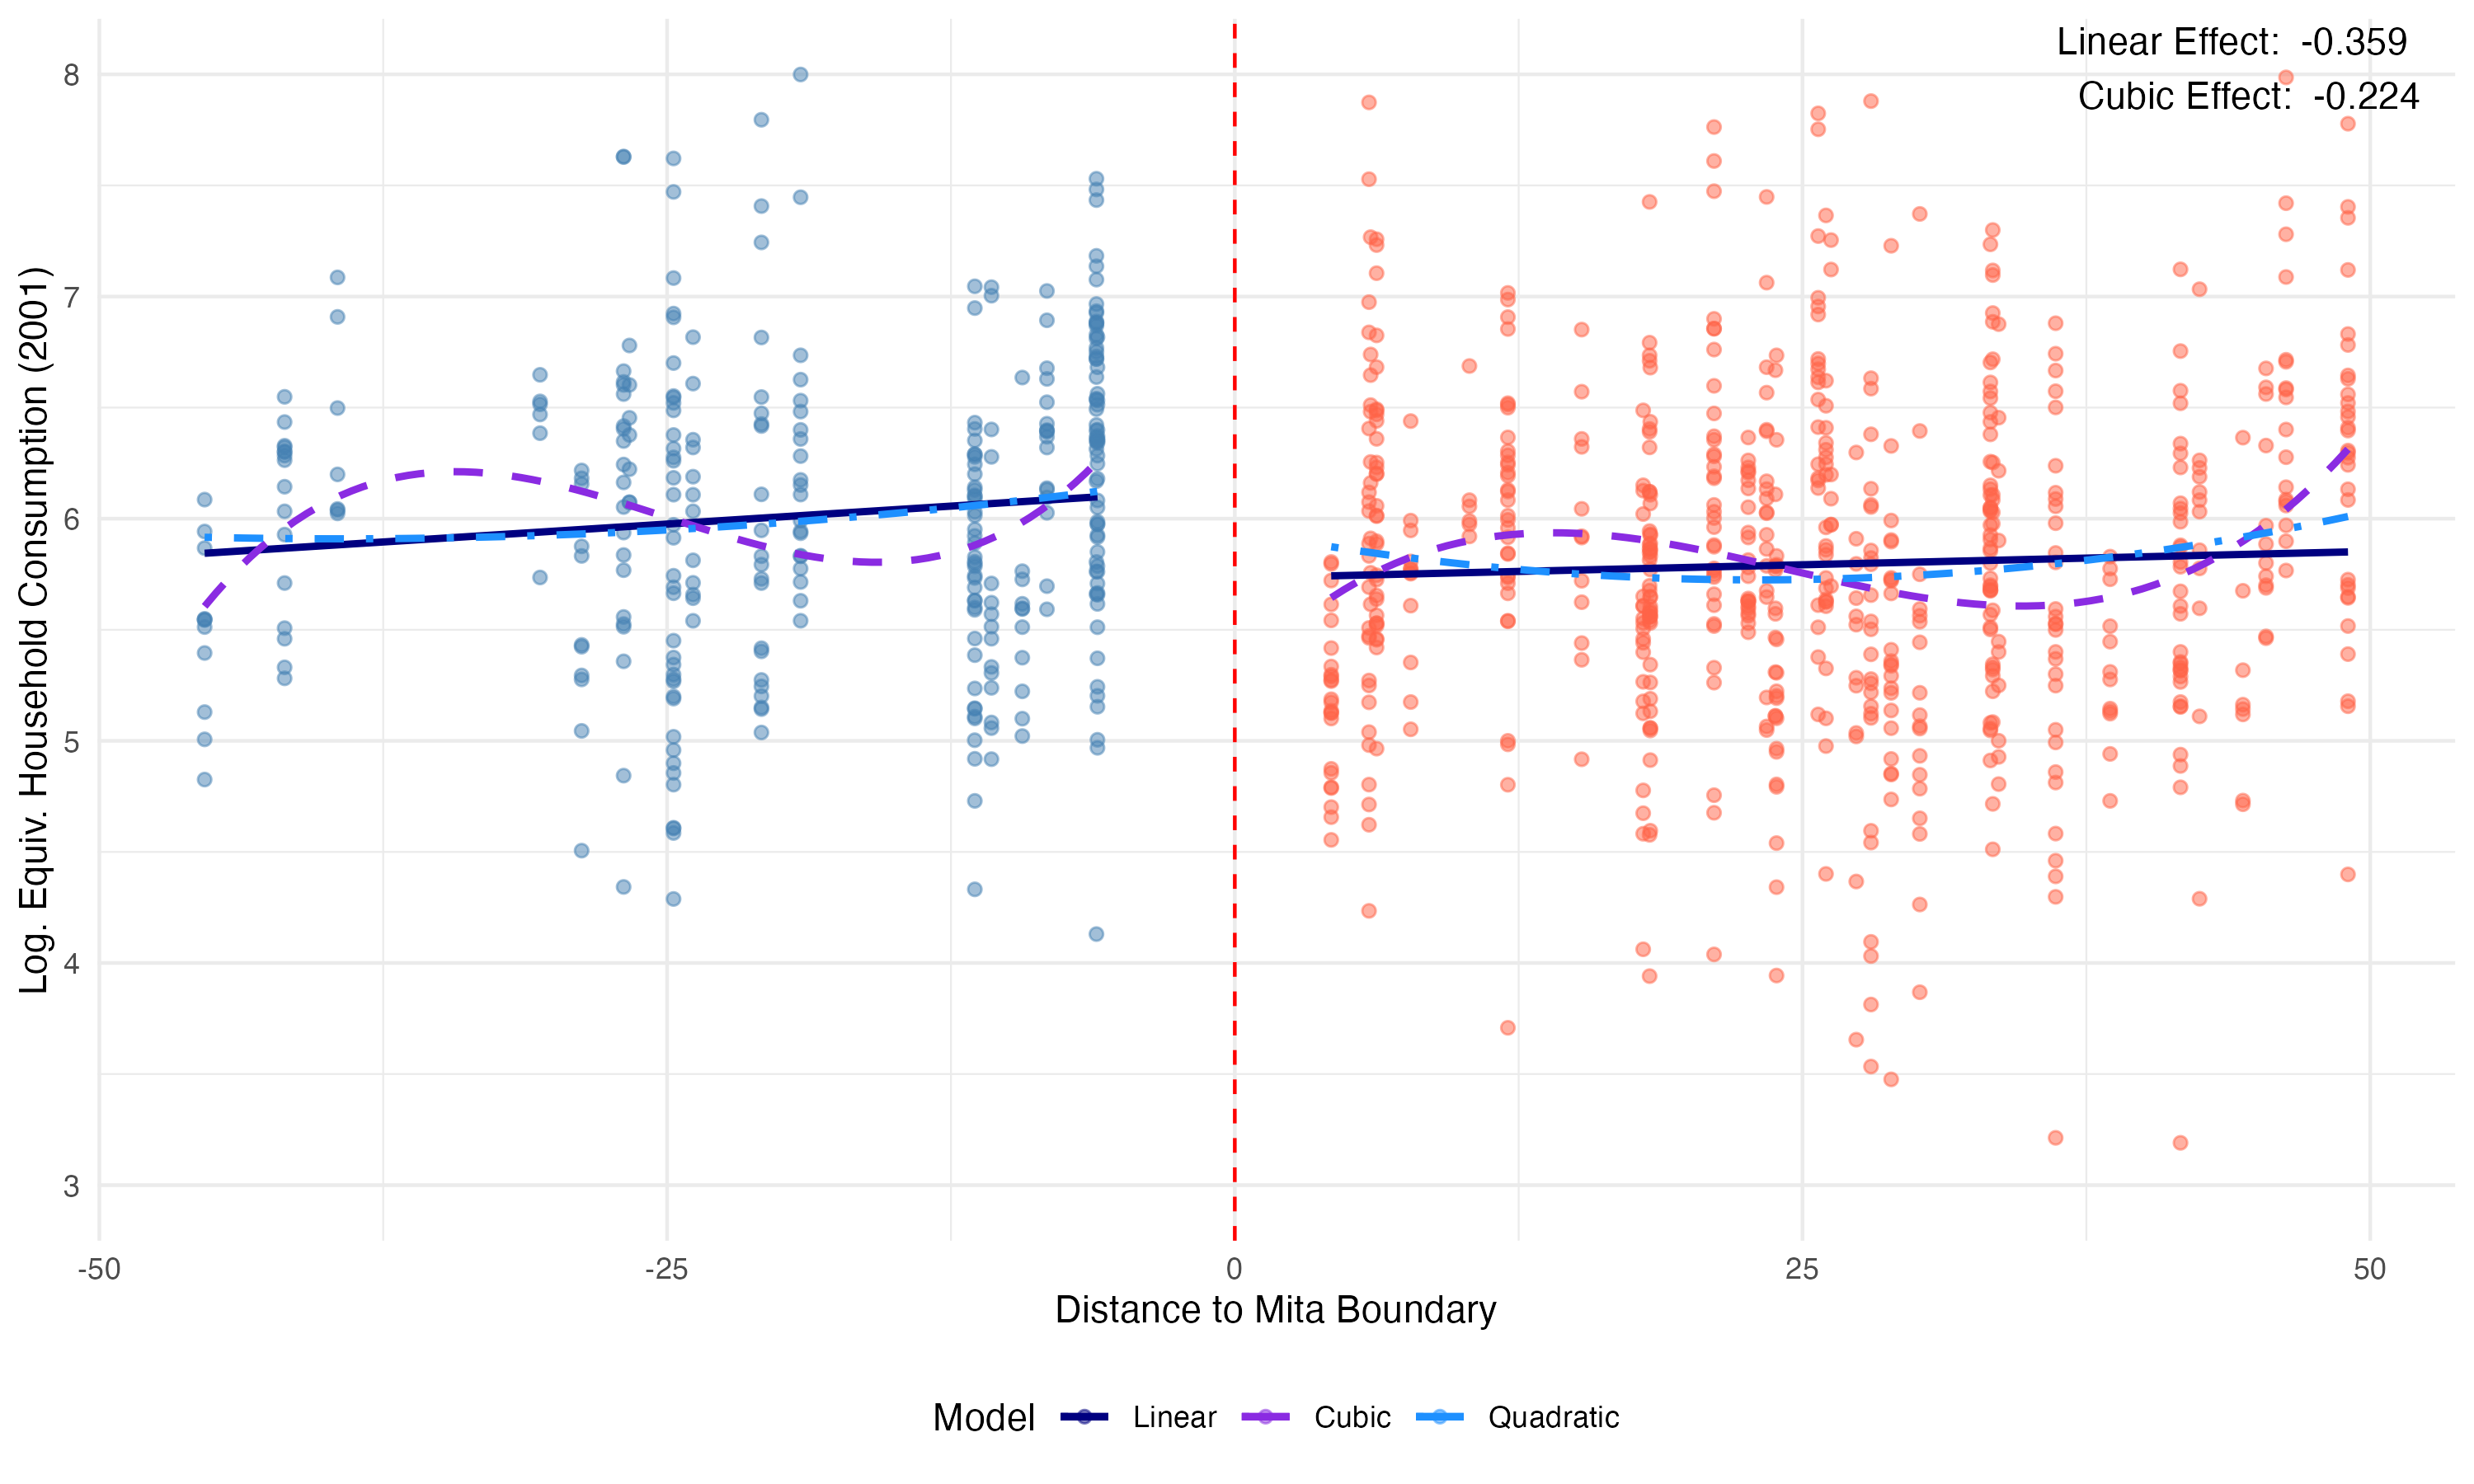
\includegraphics[width=1\linewidth]{figures/rd_plot.png}
\caption{\label{fig:plot}RD plot showing the effect of the \emph{mita} on household consumption.}
\end{figure}


\afterpage{\begin{landscape}

\subsection{Table 2: Regression Results}

Replicated Table 2 from \autocite{Dell2010Mita}.

\small 
\setlength{\tabcolsep}{3pt} 

\setlength{\LTpost}{0mm}
\begin{longtable}{l*{7}{p{0.2\textwidth}}} 
\toprule
 & \multicolumn{3}{c}{Log. Equiv. Household Consumption (2001)} & \multicolumn{4}{c}{Stunted Growth, Children 6-9 (2005)} \\ 
\cmidrule(lr){2-4} \cmidrule(lr){5-8}

% Table 1: Lat.-Long.
 & (1)\textsuperscript{\textit{1}} & (2)\textsuperscript{\textit{1}} & (3)\textsuperscript{\textit{1}} & (4)\textsuperscript{\textit{1}} & (5)\textsuperscript{\textit{1}} & (6)\textsuperscript{\textit{1}} & (7)\textsuperscript{\textit{1}} \\ 
\multicolumn{8}{c}{\textbf{Latitude and Longitude}} \\
\midrule
Mita & -0.284 & -0.216 & -0.331 & 0.070 & 0.084+ & 0.087+ & 0.114* \\ 
 & (0.199) & (0.207) & (0.219) & (0.043) & (0.046) & (0.048) & (0.049) \\ 
Num.Obs. & 1478 & 1161 & 1013 & 158848 & 115761 & 100446 & 37421 \\ 
R2 & 0.059 & 0.060 & 0.069 & 0.051 & 0.020 & 0.017 & 0.050 \\ 
\midrule

% Table 2: Potosí
\multicolumn{8}{c}{\textbf{Potosí}} \\
\midrule
Mita & -0.337*** & -0.307** & -0.329** & 0.080*** & 0.078*** & 0.078** & 0.063+ \\ 
 & (0.087) & (0.101) & (0.096) & (0.021) & (0.022) & (0.024) & (0.032) \\ 
Num.Obs. & 1478 & 1161 & 1013 & 158848 & 115761 & 100446 & 37421 \\ 
R2 & 0.046 & 0.036 & 0.047 & 0.049 & 0.017 & 0.013 & 0.047 \\ 
\midrule

% Table 3: Mita
\multicolumn{8}{c}{\textbf{Mita}} \\
\midrule
Mita & -0.277*** & -0.230* & -0.224* & 0.073** & 0.061** & 0.064** & 0.055+ \\ 
 & (0.078) & (0.089) & (0.092) & (0.023) & (0.022) & (0.023) & (0.030) \\ 
Num.Obs. & 1478 & 1161 & 1013 & 158848 & 115761 & 100446 & 37421 \\ 
R2 & 0.044 & 0.042 & 0.040 & 0.040 & 0.015 & 0.013 & 0.043 \\ 
\bottomrule
\label{tab:table2}
\end{longtable}
\begin{minipage}{\linewidth}
\textsuperscript{\textit{1}}Robust standard errors, clustered by district, are in parentheses\\
+ p \textless 0.1, * p \textless 0.05, ** p \textless 0.01, *** p \textless 0.001\\
All regressions include controls for elevation and slope, as well as boundary segment fixed effects. Columns 1–3 include demographic controls for the number of children, and adults in the household.
\end{minipage}

\end{landscape}}

\subsection{Extension: Testing  for Spatial Auto-correlation}
\label{sec:ext}

One common (one could say, 'persistent') critique of the historical persistence literature is that the results are not robust to spatial auto-correlation. In the context of this literature, the problem of spatial auto-correlation arises when the spatial arrangement of historical variables (like institutions, events, or policies) influences current outcomes in a correlated manner across geographic areas. This can lead to biased estimates if the spatial dependencies are not appropriately accounted for. In the words of Tobler's First Law of Geography, "everything is related to everything else, but near things are more related than distant things" \autocite{Tobler1970ARegion}. For instance, given that income is higher in Europe than Africa, any variable that is high in the former and low in the latter will appear to explain growth and poverty. In the context of \autocite{Dell2010Mita}, this is critical because the effect Dell argues for is institutional rather than geographic. It is the system of extraction created by the \emph{mita} that drives contemporary outcomes, not where the \emph{mita} were \emph{per se}. Spatial auto-correlation occurs when the regression residuals display a high level of correlation. Spatial auto-correlation could have the effect of driving $t$ statistics high (a common and surprising finding in much of the persistence literature). This critique has been developed in, \emph{inter alia}, \autocite{Kelly2019ThePersistence} and \autocite{Kelly2020UnderstandingPersistence}. 

Dell does go some way to account for spatial auto-correlation. Indeed, the two baseline specifications give some confidence that the results are not the pure result of spatial auto-correlation. Dell also uses robust clustered standard errors at the district level, that help control for similarities between neighbouring areas. As \autocite{Kelly2019ThePersistence} however notes, this mitigation is only meaningful insofar as the residuals are uncorrelated between clusters, which is not typically the case for spatial data.

One way to test for spatial auto-correlation is to compute the Moran statistic. The Moran statistic \autocite{Moran1950NotesPhenomena} is a measure used in spatial statistics to determine the degree of spatial auto-correlation. I compute Moran statistics for the three panel specifications, at the \textless50km bandwidth, and for the household consumption dependent variable, using the following method. The result are included below in Table \ref{tab:moran}.

\textbf{(1) Computing the spatial weights matrix:} The first step involves defining the spatial relationships between different data points. This is done by creating a 'neighbours list', which identifies which data points are considered neighbours of each other. I compute this by first producing a neighbours list using the latitude and longitude data. The neighbour list computes the $k$ nearest other observations ($k$ neighbours = 5, per \autocite{Kelly2020UnderstandingPersistence}) in Euclidean space. This is computed using great circle distance between two points $i$ and $j$ such that:
\begin{equation} \label{eq:2}
 d_{ij} = R * arcos[cos(\Delta Lon)\times sin(Lat_{r(j)})+cos(Lat_{r(i)})\times cos(Lat_{r(j)})]
\end{equation}
   
where subscripts $d$ and $r$ refer to degrees and radians, $\Delta Lon = Lon_r(j) - Lon_r(i)$ and $R$ is the radius of the earth. Each observation is connected to its k closest neighbours, forming a network of spatial relationships. These connections are then used to construct the spatial weights matrix, where the weights represent the strength or presence of a spatial relationship between each pair of observations. An $N \times N$ matrix, $W$, is formed where the element $W_{ij}$ expresses connectivity between the $i^{th}$ and $j^{th}$ area, defined as a binary if an element is a neighbour (i.e. whether it is on its neighbour list) and zero otherwise. The rows are then normalised. The diagonal elements of $W$ are by definition all zero.  
   
\textbf{Computing Moran's I:} The Moran's I statistic is then computed in the form:

\begin{equation} \label{eq:3}
I=\frac{n}{W} \frac{\sum_i \sum_j w_{i j}\left(x_i-\bar{x}\right)\left(x_j-\bar{x}\right)}{\sum_i\left(x_i-\bar{x}\right)^2}
\end{equation}

where $n$ is the number of locations, $W$ is the sum of all weights, $w_{i j}$ is the weight between locations $i$ and $j, x_i$ and $x_j$ are the standardized values of the variable at locations $i$ and $j$, and $\bar{x}$ is the mean of the variable. The formula is essentially a ratio, where the numerator captures the product of the deviation of each observation from the mean and the deviation of its neighbours (weighted by the spatial weights matrix), and the denominator is the total variance of the variable. A positive Moran's I indicates positive spatial auto-correlation (similar values cluster together), while a negative Moran's I indicates negative spatial auto-correlation (dissimilar values cluster together). 

\textbf{Applying Moran statistics:} In the context of Dell's analysis, the presence of spatial auto-correlation would suggest that there are spatial patterns in the data that are not random. This could mean that the effects of the \emph{mita} system are spatially varying and possibly correlated with other regional characteristics or unobserved variables. The results at Table \ref{tab:moran} suggest that low-to-moderate spatial auto-correlation is a potential issue with the analysis. I have visualised the result for the 50km bandwidth in Figure \ref{fig:moran} contained in the Appendix (\ref{sec:appendix}). The figure shows the Moran statistic as the slope of the line that best fits the relationship between each observation's household consumption and spatially lagged counterparts. 

Across all three models, the Moran statistics are positive and significant, ranging from $0.093$ to $0.125$.\footnote{As weights and the variable of interest are standardised in this analysis, the Moran statistic is bounded $[-1, 1]$, with $-1$ denoting perfectly negative spatial auto-correlation and $1$ perfectly positive spatial auto-correlation. A value of $0$ would represent a random geographic distribution.} The expected value is $\approx 0$, which aligns with the expectation of random spatial distribution under the null hypothesis. Nearby observations tend to have more similar residual values than would be expected if there were no spatial auto-correlation. This would tentatively support the critique from \autocite{Kelly2019ThePersistence} and \autocite{Kelly2020UnderstandingPersistence} that persistence regressions do not contain adequate controls for unobserved spatially-correlated variables, suggesting the causal claim made regarding the institutional effect of the \emph{mita} may not be as significant as first thought.

Spatial auto-correlation does not necessarily invalidate Dell's findings but highlights the need for careful interpretation. It suggests that additional spatial factors might be influencing the outcomes, and these should be accounted for in the analysis. The auto-correlation might occur for a host of reasons, for instance, if regions closer to ancient mines, irrespective of the \emph{mita} influence, have developed distinct economic characteristics due to factors like mineral wealth. This could create a pattern where neighbouring regions have similar economic outcomes, not directly due to the \emph{mita}, but because of their proximity to mines. This is however speculation and lends itself to further investigation. 

\section{Conclusion}
\autocite{Dell2010Mita} provides one of the most important results in the historical persistence literature, demonstrating the long-term and significant effect of extractive economic institutions on contemporary living standards. These results are consistent across household consumption and childhood stunting and are robust to a range of specifications. Building on \autocite{Kelly2019ThePersistence}, I extend Dell's analysis to test whether the results are robust to spatial auto-correlation, finding evidence of low-to-medium spatial auto-correlation. This suggests that there may be confounding geographic factors that could at least partially explain Dell's results.

\pagebreak
\section{Appendix} \label{sec:appendix}

\begin{longtable}{lrrr}
\caption*{
{Table \ref{tab:moran}: Moran's I Test Results for Spatial Auto-correlation}
} \\ 
\toprule
Model & Moran's I & P-value & Expected Value \\ 
\midrule
Latitude-Longitude Model & $0.071$ & $0.000$ & $-0.001$ \\ 
Potosi Model & $0.097$ & $0.000$ & $-0.001$ \\ 
Mita Model & $0.099$ & $0.000$ & $-0.001$ \\ 
\bottomrule
\label{tab:moran}
\end{longtable}

\begin{figure}[H] 
\centering
\title{Figure \ref{fig:map}: The \emph{mita} region of Peru and Bolivia}\par\medskip
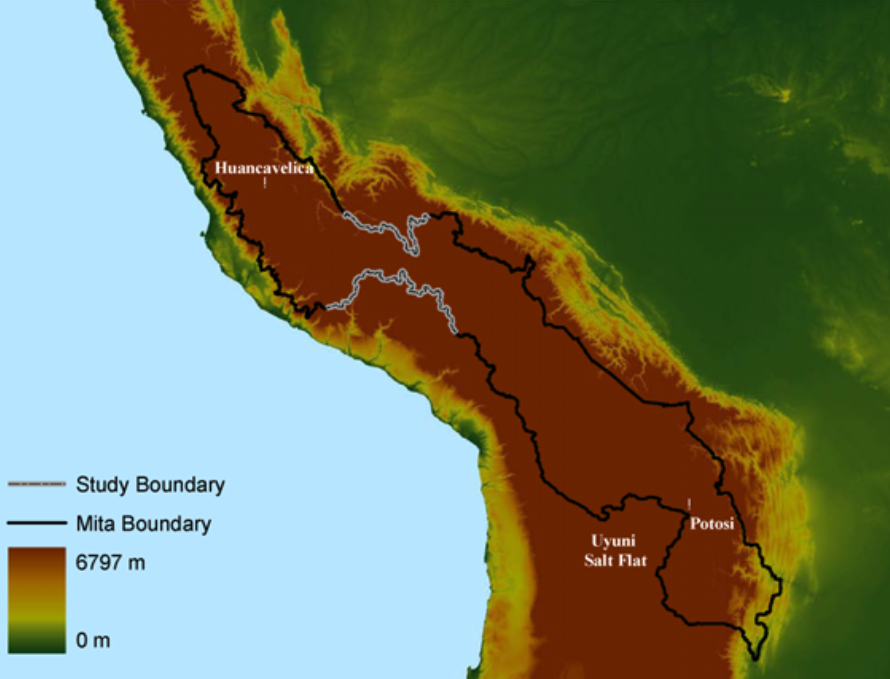
\includegraphics[width=1\linewidth]{figures/fig1_map.png}
\caption{\label{fig:map}The \emph{mita} boundary is in black. The study boundary is in light grey. The map also shows elevation across the area of interest. Source: \autocite{Dell2010Mita}.}
\end{figure}


\begin{figure}[H]
\centering
\title{Figure \ref{fig:moran}: Visualising Moran statistics}\par\medskip
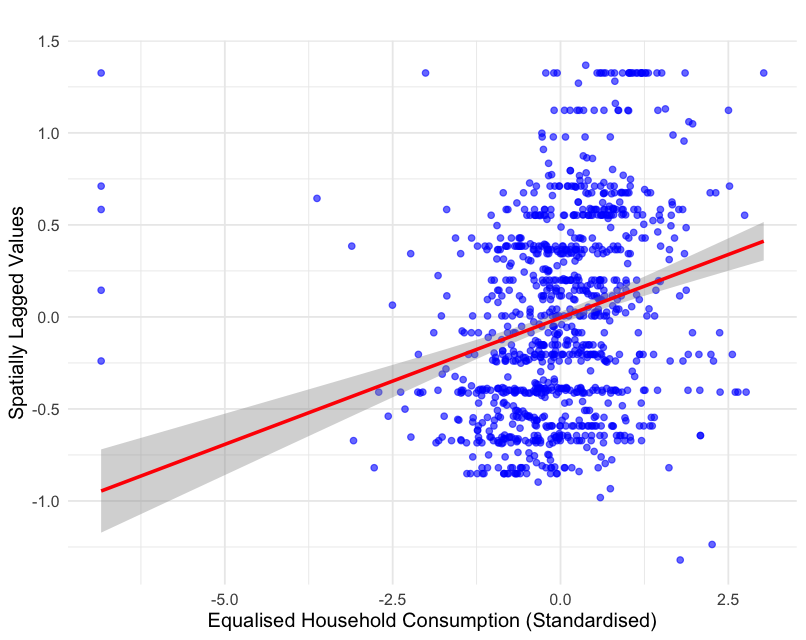
\includegraphics[width=1\linewidth]{figures/moran.png}
\caption{The plot shows spatially lagged values of standardised household consumption correlated with non-lagged values, for the \textless 50km bandwidth. This visually shows the Moran statastic, which is essentially the slope of this graph.}
\label{fig:moran}
\end{figure}


\pagebreak
\printbibliography 

\end{document}